\section{A word about automatic differentiation}
\label{sec:word-about-automatic}
The transposition principle has often been viewed as a special case of
the reverse mode in automatic differentiation
\cite{KY88,Ka2K,BoLeSc03}. This is somewhat ironic as the whole idea
of automatic differentiation can elegantly be derived in the
arithmetic circuit model and reverse mode in particular is just an
application of the transposition principle \cite{GG05}. It is probable
that the need for efficient AD tools in many scientific areas other
than mathematics and computer science is responsible for such reversal
of roles.

In this section we show how AD can be expressed in the arithmetic
circuit model and then discuss the main differences between the AD
tools and our approach. A more complete study on the differentiation
of circuits and on how the transposition principle relates the
gradient to the differential can be found in \cite{GG05,Ser08}, of
which this Section is a simplification.

To simplify the presentation, we consider a basis $\mathcal{B}$ over
$\R$ made exclusively of everywhere continuously derivable functions
(w.r.t the standard metric of the Euclidean space $\R^n$). What we
give here is a technique to approximate a circuit over
$(\R,\mathcal{B})$ by a ``linear'' circuit.

\begin{definition}[Derivative of a circuit]
  Let $C$ be a circuit over $(\R,\mathcal{B})$ with $n$ inputs and let
  $x\in\R^n$. For any function $f\in\mathcal{B}$, we note by $J_f$ its
  Jacobian. Then the \emph{derivative} of $C$ at $x$, noted $\diff_x
  C$ is the arithmetic circuit where any $v\in V$ with $\beta(v)=f$
  and incident edges $e_1,\ldots,e_m$ has been substituted by a $v'$
  with
  \begin{equation}
    \label{eq:derivative}
    \beta(v')=J_f\left(\eval_{e_1}(x),\ldots,\eval_{e_m}(x)\right)
    \text{ .}
  \end{equation}
\end{definition}

\begin{figure}[!ht]
  \centering
  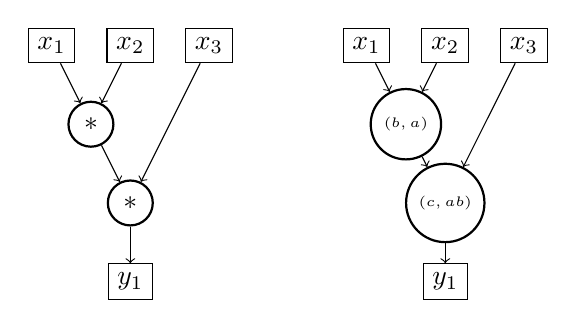
\begin{tikzpicture}
    \tikzstyle{node}=[circle,thick,draw=black,minimum size=4mm]
    \tikzstyle{arg}=[rectangle,thin,draw=black,minimum size=4mm]
    
    \begin{scope}
      \node[arg](in1){$x_1$};
      \node[arg,right of=in1](in2){$x_2$};
      \node[arg,right of=in2](in3){$x_3$};
      \node[node,below of=in1,xshift=5mm](times1){$*$};
      \node[node,below of=times1,xshift=5mm](times2){$*$};
      \node[arg,below of=times2](out){$y_1$};

      \path[->]
      (in1) edge (times1)
      (in2) edge (times1)
      (times1) edge (times2)
      (in3) edge (times2)
      (times2) edge (out);
    \end{scope}

    \begin{scope}[xshift=4cm]
      \node[arg](in1){$x_1$};
      \node[arg,right of=in1](in2){$x_2$};
      \node[arg,right of=in2](in3){$x_3$};
      \node[node,below of=in1,xshift=5mm](times1){\tiny$(b,a)$};
      \node[node,below of=times1,xshift=5mm](times2){\tiny$(c,ab)$};
      \node[arg,below of=times2](out){$y_1$};

      \path[->]
      (in1) edge (times1)
      (in2) edge (times1)
      (times1) edge (times2)
      (in3) edge (times2)
      (times2) edge (out);
    \end{scope}
  \end{tikzpicture}
  \caption{A circuit and its derivative at the point $x=(a,b,c)$.}
  \label{fig:derivative}
\end{figure}

Taking the derivative of a circuit at $x$ amounts to chose for each
node the best linear approximation at the point where it is
evaluated. It is clear that this yields the best linear approximation
for the circuit at $x$.

\begin{proposition}
  $\eval_{\diff_xC}=J_{\eval_C}(x)$.
\end{proposition}

It is also clear that $\diff_xC$ is defined over a basis that is
exclusively made of matrices with coefficients in $\R$, in other words
$\diff_xC$ is defined in $RMod{\R}$. We have thus defined a
transformation from black-box derivable functions to black-box
matrices.

Now the black-box $\diff_xC$ can be queried by black-box algorithms to
obtain information about the Jacobian. The most simple application is
to compute the directional derivative in $x$ along a direction $u$:
for this task it suffices to evaluate the circuit once since
$\eval_{\diff_xC}(u)$ is the desired value. Computing the derivative
along $n$ linearly independent directions yields the whole Jacobian
and this corresponds to the direct mode in automatic
differentiation\footnote{To be more precise, direct mode automatic
  differentiation constructs $\diff_xC$ and evaluates the $n$
  directions in parallel, thus reducing the amount of storage
  needed.}.

When the circuit has many inputs but only one output, there is a more
convenient way to get the whole gradient with only one black-box
query: $\diff_xC$ computes a linear form whose coefficients are
exactly the coefficients of the gradient, thus the dual circuit
$\dual{(\diff_xC)}$ computes the transposed form\footnote{We haven't
  actually proven the transposition theorem for an arbitrary basis,
  but it should be clear how to generalize it.}, or column vector. The
single query $\eval_{\dual{(\diff_xC)}}(1)$ yields this vector. This
is exactly what is called ``reverse mode'' in automatic
differentiation.

Note however that one is not limited to direct or reverse mode: any
black-box algorithm can be combined with the derivative circuit to
obtain information on the original function. For example Wiedemann's
algorithm \cite{Wie86} can be used to determine if the function is
invertible around $x$ and directional derivatives of the inverse can
be computed.

Of course, direct and reverse automatic differentiation can be defined
by the more classical chain rule, and then the transposition theorem
can be derived as a special case of the reverse mode by observing
that, when all the nodes of the circuit are linear maps, $C=\diff_xC$
for any $x$. After all, the code transformation techniques given in
\cite{BoLeSc03} and further developed in Section \ref{sec:} were
already invented by researchers in AD \cite{GVM91}, though not often
implemented. 

This being said, why treat transposition separately?  The answer is
manifold and we only list here some key points.
\begin{itemize}
\item AD is often interested in recovering the full Jacobian, instead
  of just having a black-box for it. For an $n\times m$ matrix, this
  requires $n$ queries in direct mode or $m$ queries in reverse
  mode. In both cases, AD tools do more work than what we would like
  to.
\item Many AD tools do not optimize the computation of $\diff_xC$ for
  the case where nodes are linear and still compute the whole
  circuit. In particular, many AD tools generate a graph
  representation of an arithmetic circuit from a program instead of
  directly transposing the code. This adds a constant overhead to the
  case of transposition where simply $\diff_xC=C$.
\item If the circuit $\diff_xC$ is computed, it must be fully stored
  in memory for reverse mode. This may seem innocuous as $\diff_xC$
  has the same size as $C$, but consider programs that compute
  $\eval_C$ by means of for loops or other iterative constructs: while
  the evaluation of $C$ is compact and cheap, the evaluation of
  $\diff_xC$ possibly requires to introduce a new variable for each
  iteration of the loop. Depending on the implementation, this may
  lead to code or storage bloat. In the case of transposition, this
  never happens since for loops are directly reversed (at least when
  all the variables are linear). Griewank \cite{Gri92} gives a
  time/memory compromise that permits to keep both storage and time in
  a factor of $\log n$ from the original program, but this is still
  not as good as transposition.
\item Our approach is more general in that it permits to automatically
  treat functions that depend both on linear and non-linear arguments
  without any help from the user. Thanks to this, we are able to treat
  recursive functions, while, to the extent of our knowledge, no AD
  tool can.
\item Our approach is algebraic and permits to prove bounds on the
  algebraic complexity of the generated programs, while AD tools
  usually only deal with floating point numbers. More generally, AD
  languages are usually less rich than \tAL.
\end{itemize}




% Local Variables:
% mode:flyspell
% ispell-local-dictionary:"american"
% mode:TeX-PDF
% mode:reftex
% TeX-master: "../these"
% End:
%
